\documentclass[11pt, oneside]{article} 
\usepackage{geometry}
\geometry{letterpaper} 
\usepackage{graphicx}
	
\usepackage{amssymb}
\usepackage{amsmath}
\usepackage{parskip}
\usepackage{color}
\usepackage{hyperref}

\graphicspath{{/Users/telliott/Dropbox/Github-Math/geoproof/figures/}{/Users/telliott/Dropbox/Github-Math/figures/}}
% \begin{center} \includegraphics [scale=0.4] {gauss3.png} \end{center}


\title{Parallelogram}
\date{}

\begin{document}
\maketitle
\Large

%[my-super-duper-separator]

So far we have dealt mainly with triangles.  Triangles are members of the first of two large categories of shapes in geometry, namely polygons, which have straight sides, and curves.  Polygons are composed of line segments, and curves include circles as well as various conic sections like the ellipse, the parabola, and so on.

Triangles are polygons with three sides, of course.  Quadrilaterals have four sides.  They are in turn organized by whether one pair of opposing sides is equal, or possibly both pairs are equal, and whether the angles inside are right angles.

It is helpful to remember that any quadrilateral can be divided by a diagonal into two triangles.  As a result, we have that the total of all the angles in such a polygon is equal to four right angles, or 360.

\subsection*{parallelogram}

This chapter introduces the parallelogram.  Its theorems provide practice in the methods of proving congruence for triangles.

A parallelogram is a quadrilateral with both pairs of opposing sides equal and parallel, and both pairs of opposite angles equal.
\begin{center} 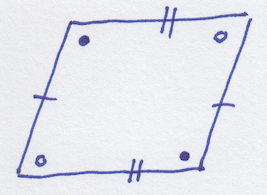
\includegraphics [scale=0.5] {F1.png} \end{center}

However, just as with congruent triangles, it is not necessary to show all these conditions are true before we can know that we have a parallelogram.

The first example is one pair of opposite sides equal and parallel.  The marked angles are equal by alternate interior angles.
\begin{center} 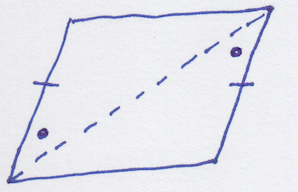
\includegraphics [scale=0.5] {F3.png} \end{center}
The two triangles formed by the diagonal are congruent by SAS.  This gives the other properties.

The second example is both pairs of opposing sides equal.
\begin{center} 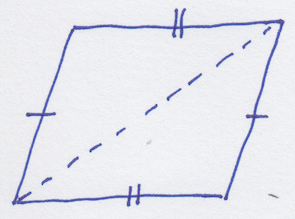
\includegraphics [scale=0.5] {F2.png} \end{center}
Here we have the third side shared, hence the two triangles formed by the diagonal are congruent by SSS.  Again, this gives the other properties.

The third case is both pairs of opposing sides parallel.
\begin{center} 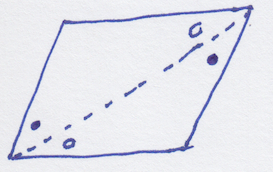
\includegraphics [scale=0.5] {F4.png} \end{center}
This gives the indicated angle equalities, which means we have congruent triangles by ASA.  This gives the rest of the equalities.

The fourth case is both pairs of opposing angles equal:
\begin{center} 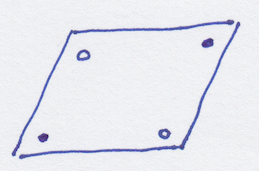
\includegraphics [scale=0.5] {F5.png} \end{center}

Any quadrilateral can be cut into two triangles, hence the sum of angles in a quadrilateral is four right angles.  Since this is equal to two pairs of equal angles, the sum of one of each pair is equal to two right angles.  Hence both pairs of opposing sides are parallel.  

Therefore, we have the third case.

The fifth and last case is one pair of opposing sides equal and parallel (refer to the diagram for the third case and make the relevant substitution).  When the diagonal is drawn we again have equal angles by alternate interior angles, and equal flanking sides, which from which it follows that the two triangles are congruent, by SAS.

The last case becomes useful later in dealing with the central theorem regarding similar triangles, due to Euclid.

\subsection*{midpoints of diagonals}

The two diagonals of a parallelogram cross at their midpoints.

The angles marked equal are equal by alternate interior angles.
\begin{center} 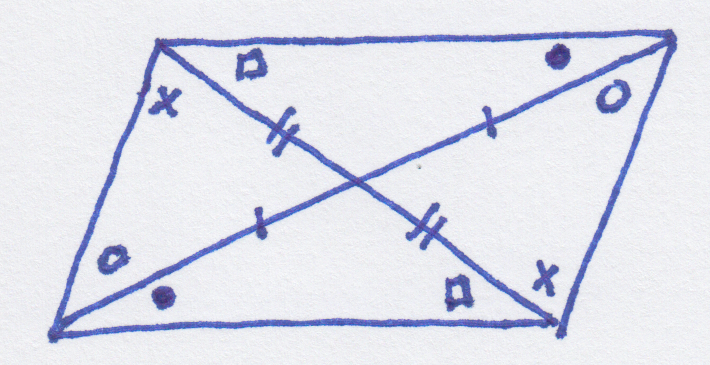
\includegraphics [scale=0.25] {F6.png} \end{center}

We have two sets of congruent triangles, by ASA (given that the opposing sides are equal).  

Therefore, each diagonal is divided in half, even though one is longer than the other.

\end{document}
